\begin{frame}
  \frametitle{Performance Analysis Using Projections}
  \begin{block}{Instrumentation and measurement during program execution}
    \begin{itemize}
        \item Easy setup: just modify link options
        \item Easy setup: data is generated automatically during run
        \item User events can be easily inserted as needed
    \end{itemize}
  \end{block}
  \begin{block}{Visualization and analysis client}
    \begin{itemize}
        \item Scalable: analyze execution traces for 100s of thousands of cores 
        \item Rich feature set: time profile, time lines, usage profile, histograms, outliers etc
        \item Detect performance problems: load imbalance, grain size, communication bottleneck, etc 
    \end{itemize}
  \end{block}
\end{frame}


\begin{frame}{Time Profile}
 \includegraphics<1>[width=0.9\textwidth]{../figures/prj1M8KTimeprofile.png}
\end{frame}

\begin{frame}{Extrema Tool for Least Idle Processors}
\includegraphics<1>[width=0.9\textwidth]{../figures/prj1M8KExtrema.png}
\end{frame}

\begin{frame}{Time Lines with Message Back Tracing}
\centering
\includegraphics<1>[width=0.9\textwidth]{../figures/prj1M8KTimeline.png}
\end{frame}


\begin{frame}{Communication over Time for all Processors}
 \includegraphics<1>[width=0.9\textwidth]{../figures/prj1M8KCommtime.png}
\end{frame}


\begin{frame}[fragile]
  \frametitle{Debugging \charm applications using CharmDebug}
  \begin{center}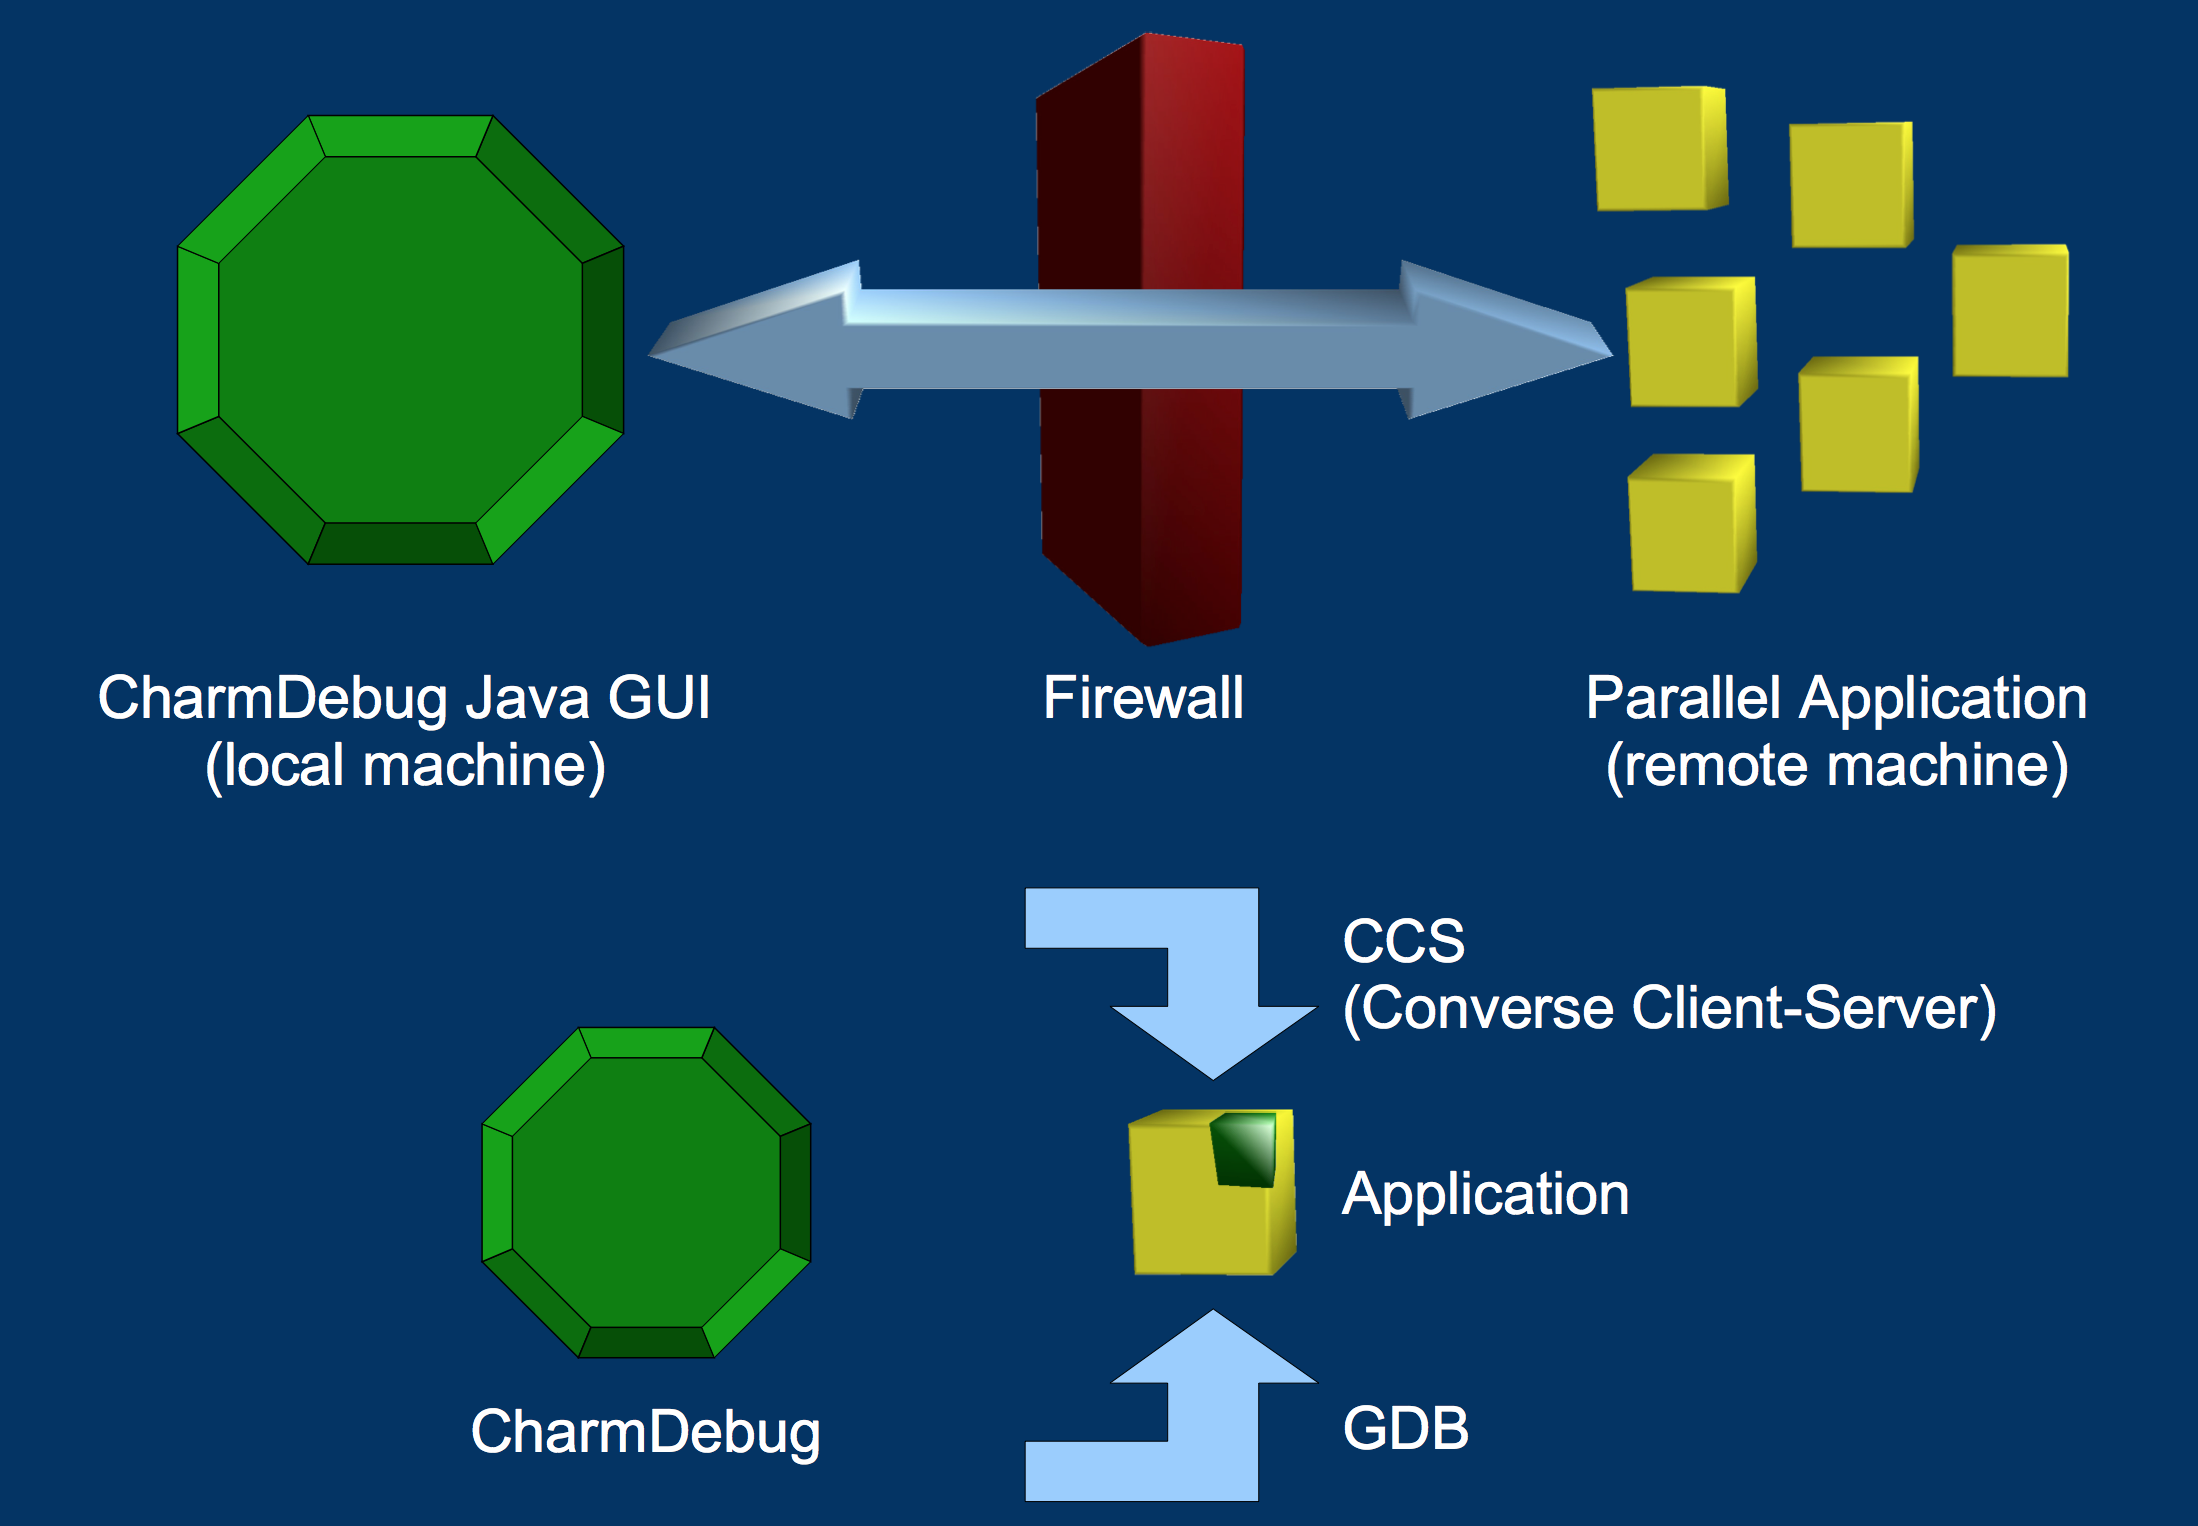
\includegraphics[width=0.9\textwidth]{../figures/overviewDebug.png}\end{center}
\end{frame}

\begin{frame}[fragile]
  \frametitle{Debugging \charm applications using CharmDebug}
  \begin{center}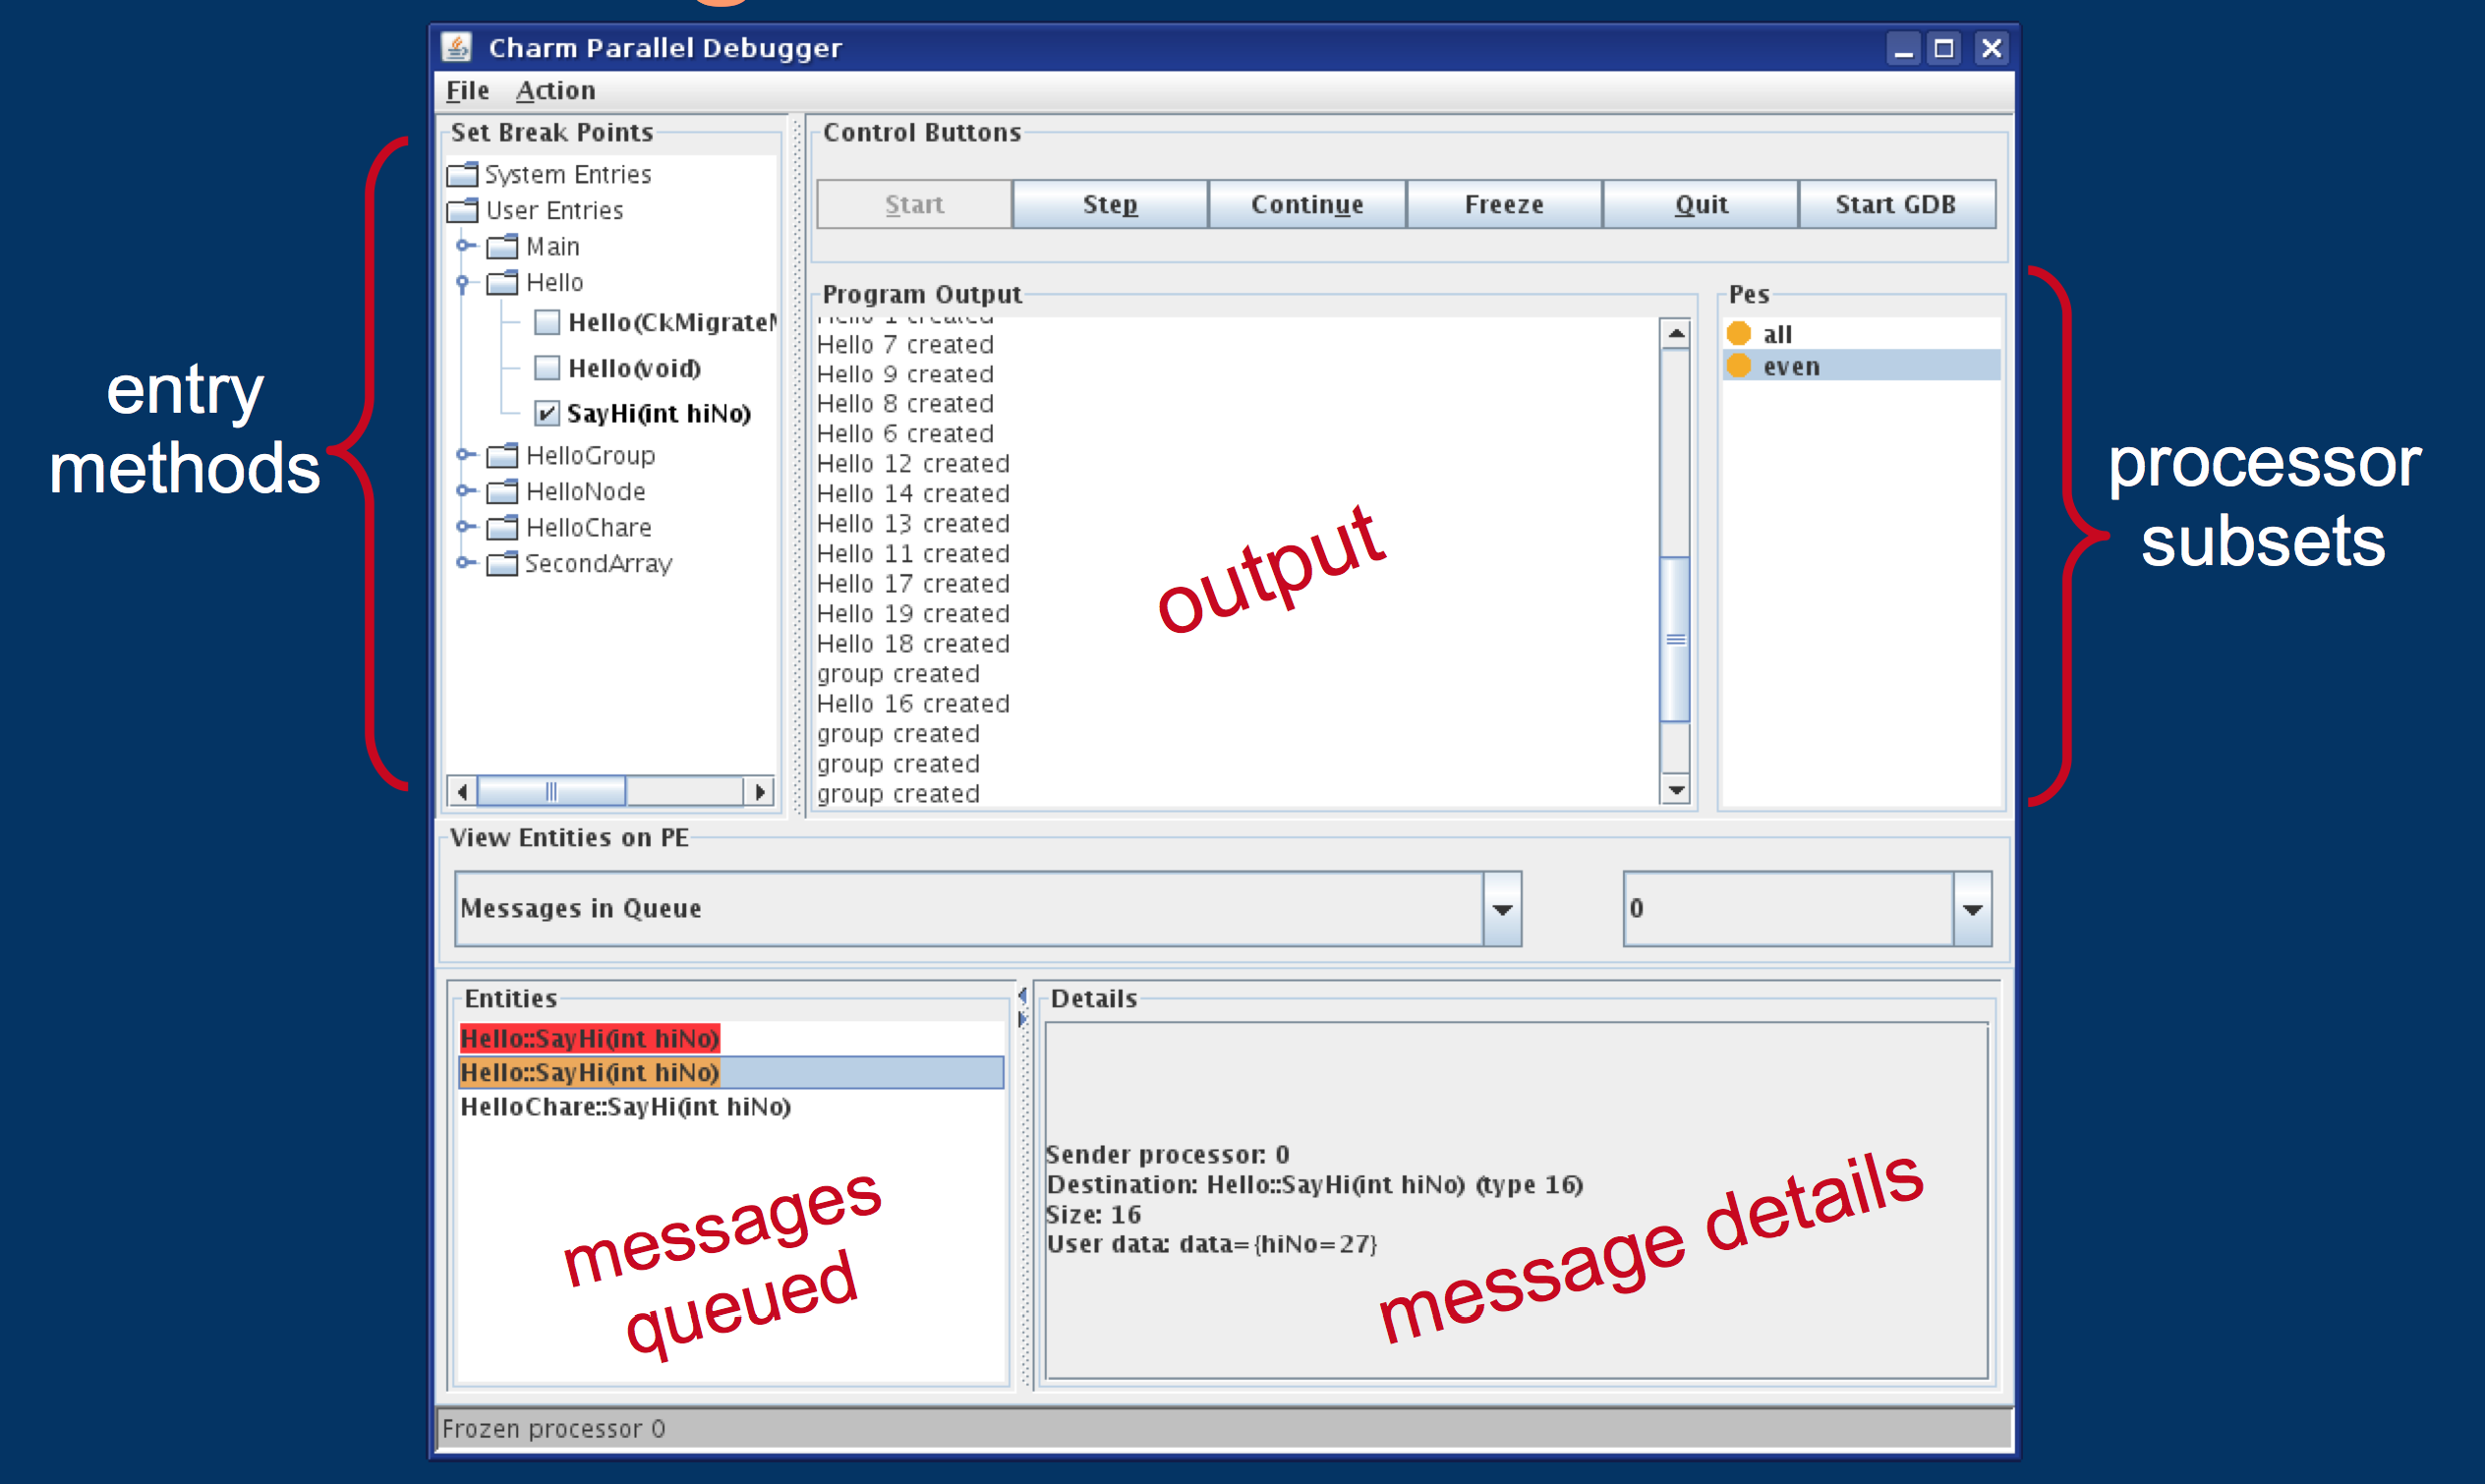
\includegraphics[width=0.9\textwidth]{../figures/debugMainView.png}\end{center}
\end{frame}

